\documentclass[../../main.tex]{subfiles}


\begin{document}

\subsection*{(a)}
There are 4982 Applications with an average throughput time of 21.904 as determined using the following Process:\\
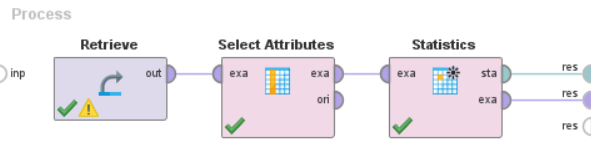
\includegraphics[width=\textwidth]{img/QUESTION_5a_PROCESS_average_throughput_time.png}

Using Celonis Process AI on our Dataset we learn that the most frequent variant (happy path) happens 320 times. This variant can be seen below.\\
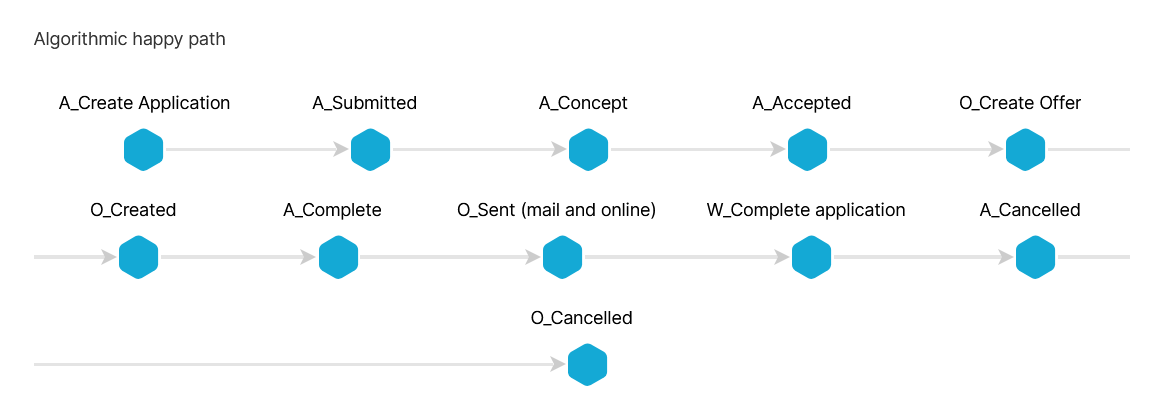
\includegraphics[width=\textwidth]{img/QUESTION_5a_happy_path.png}

The following graph shows the frequency distribution of the throughput times. As one can see they are initially quite high and eventually deteriorate in frequency until the 29-33 Day, where they spike again and after that deteriorate quickly again. The reason for the spike at 29-33 Days is probably that a new month begins/ends at this time. Therefore many applications will likely be terminated at this time for administrative reasons.\\
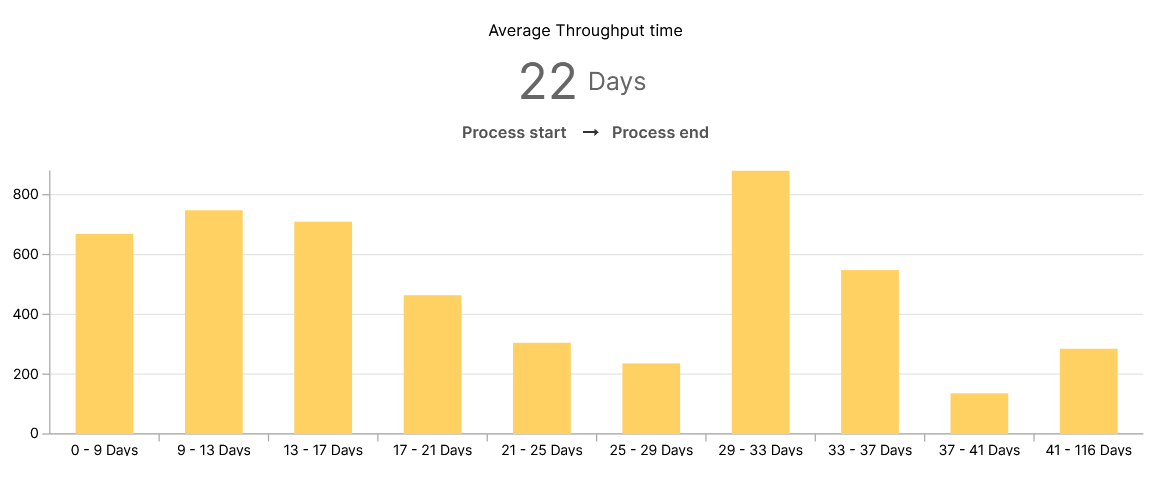
\includegraphics[width=\textwidth]{img/QUESTION_5a_throughput_time_distribution.png}



\subsection*{(b)}
The BPMN model for cases running under 30 days can be seen below (zoom in to inspect in detail). We created it by starting a new Analysis and opening a new \textit{conformance} sheet. Then we clicked \textit{Mine process model} and in the next window added a new selection for Throughput time under 30. Then we clicked \textit{select all} and \textit{Launch analysis}. We then clicked \textit{View process model} where the model below was displayed and downloadable.\\
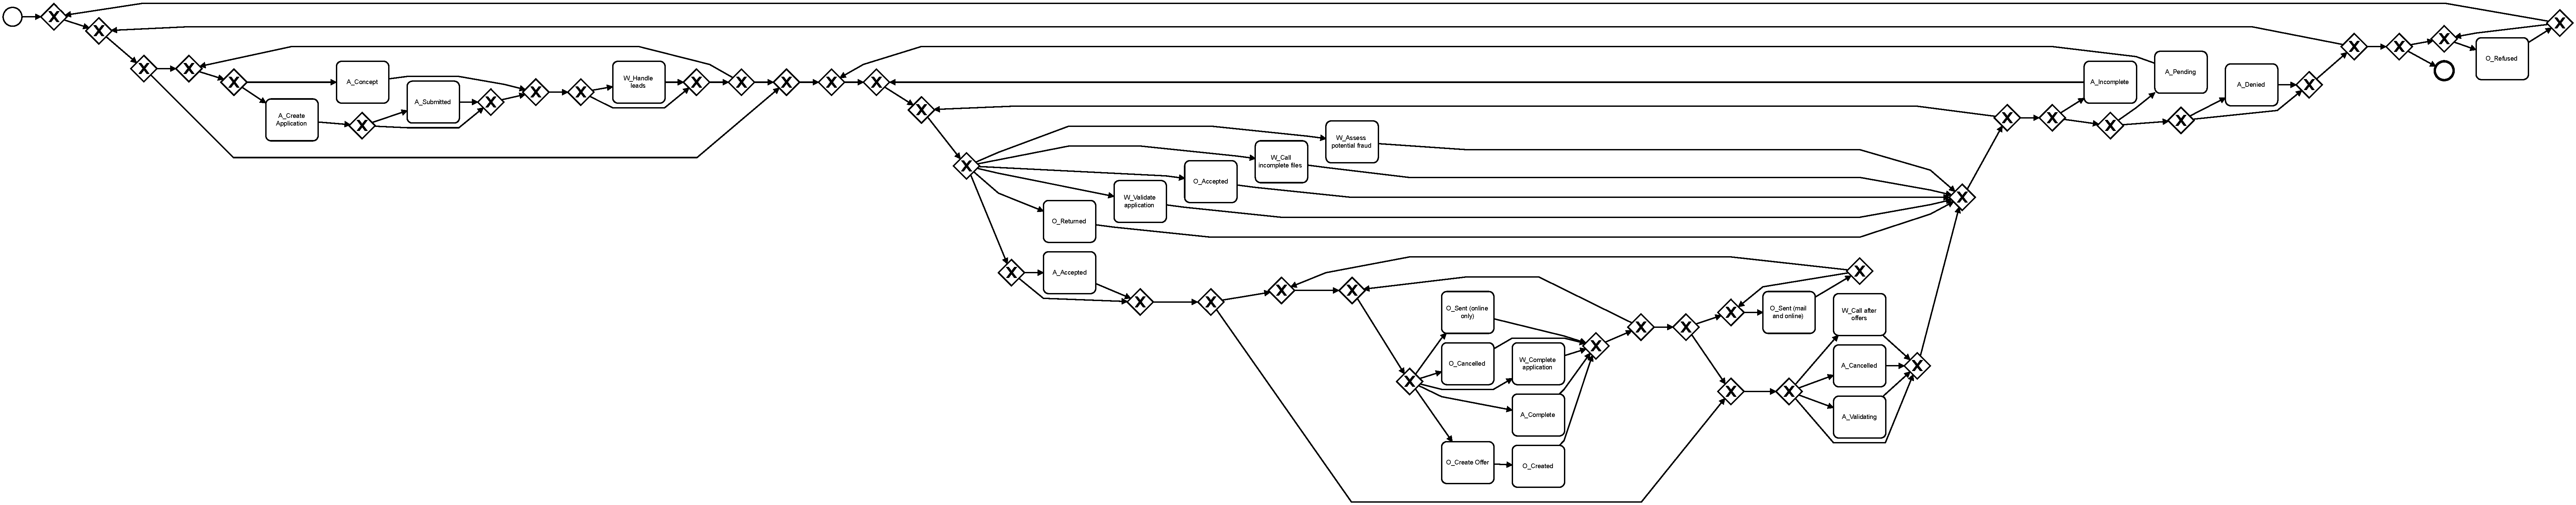
\includegraphics[width=\textwidth]{img/QUESTION_5b_BPMN_model.pdf}


\subsection*{(c)}
We open a new Process Overview for our Process in Celonis just like we did in a). To exclude all cancelled applications we add a new selection of type \textit{Attribute selection}. Since per definition cancelled applications are those that contain the activity \textit{A$\_$cancelled} we exclude all the applications containing it by selecting \texttt{Activity$\_$table$\_$csv > ACTIVITY > A$\_$Cancelled} and click \textit{Invert selection}. We also create a new throughput time selection for applications with a throughput time between 30 and infinity to only see long running cases. The resulting Process Overview can be seen below.\\
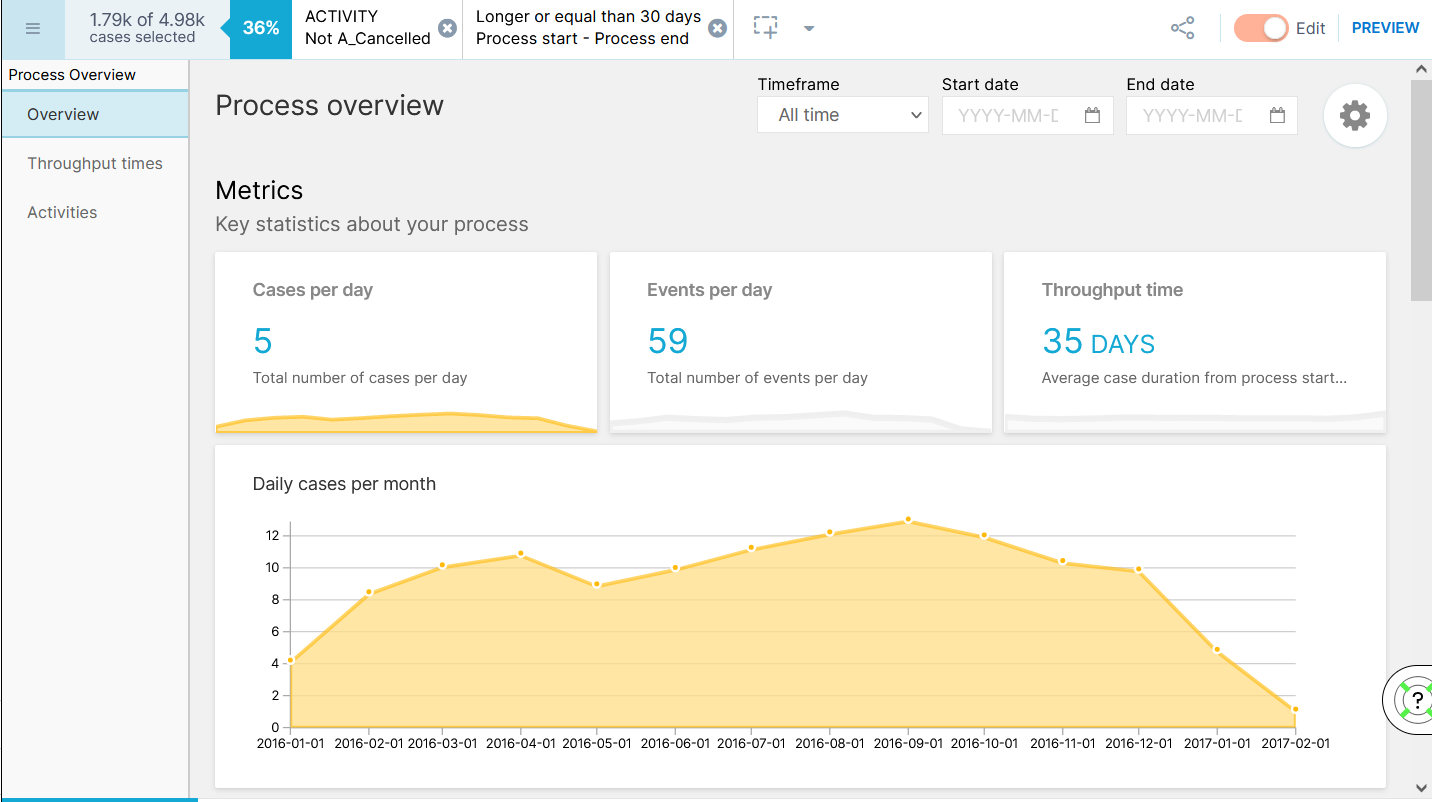
\includegraphics[width=\textwidth]{img/QUESTION_5c_process_overview.png}
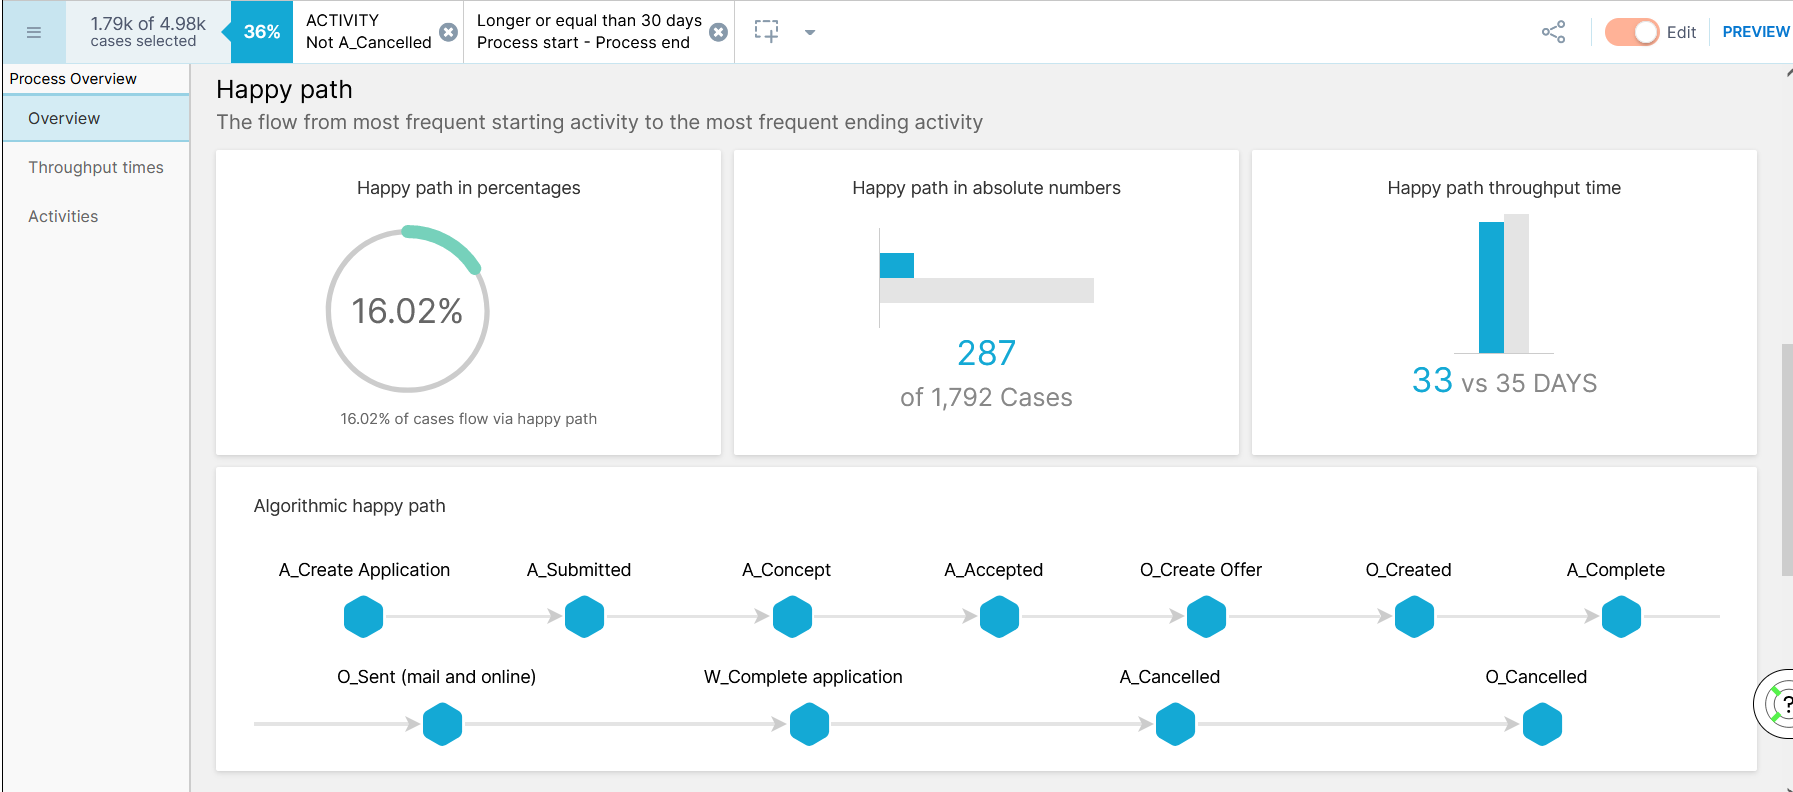
\includegraphics[width=\textwidth]{img/QUESTION_5c_process_overview_happy_path.png}
From it we learn that there are 1792 long running applications that weren't cancelled. 


\subsection*{(d)}



\end{document}